
% This LaTeX was auto-generated from an M-file by MATLAB.
% To make changes, update the M-file and republish this document.

\documentclass{article}
\usepackage{graphicx}
\usepackage{color}

\sloppy
\definecolor{lightgray}{gray}{0.5}
\setlength{\parindent}{10pt}
\usepackage[margin=1in]{geometry}

\begin{document}

\title{Dynamical Adaptation in ORNs}
\author{Srinivas Gorur-Shandilya}
\maketitle

    
    

\section*{Effect of Correlation Time on Linear Filters}

\begin{par}
What is the effect of correlation time of the stimulus on the ORN response, and the filter that we calculate from this data?
\end{par} \vspace{1em}
\begin{par}
First, we plot the autocorrelation functions of the valve, the stimulus and the ORN and check that they make sense.
\end{par} \vspace{1em}

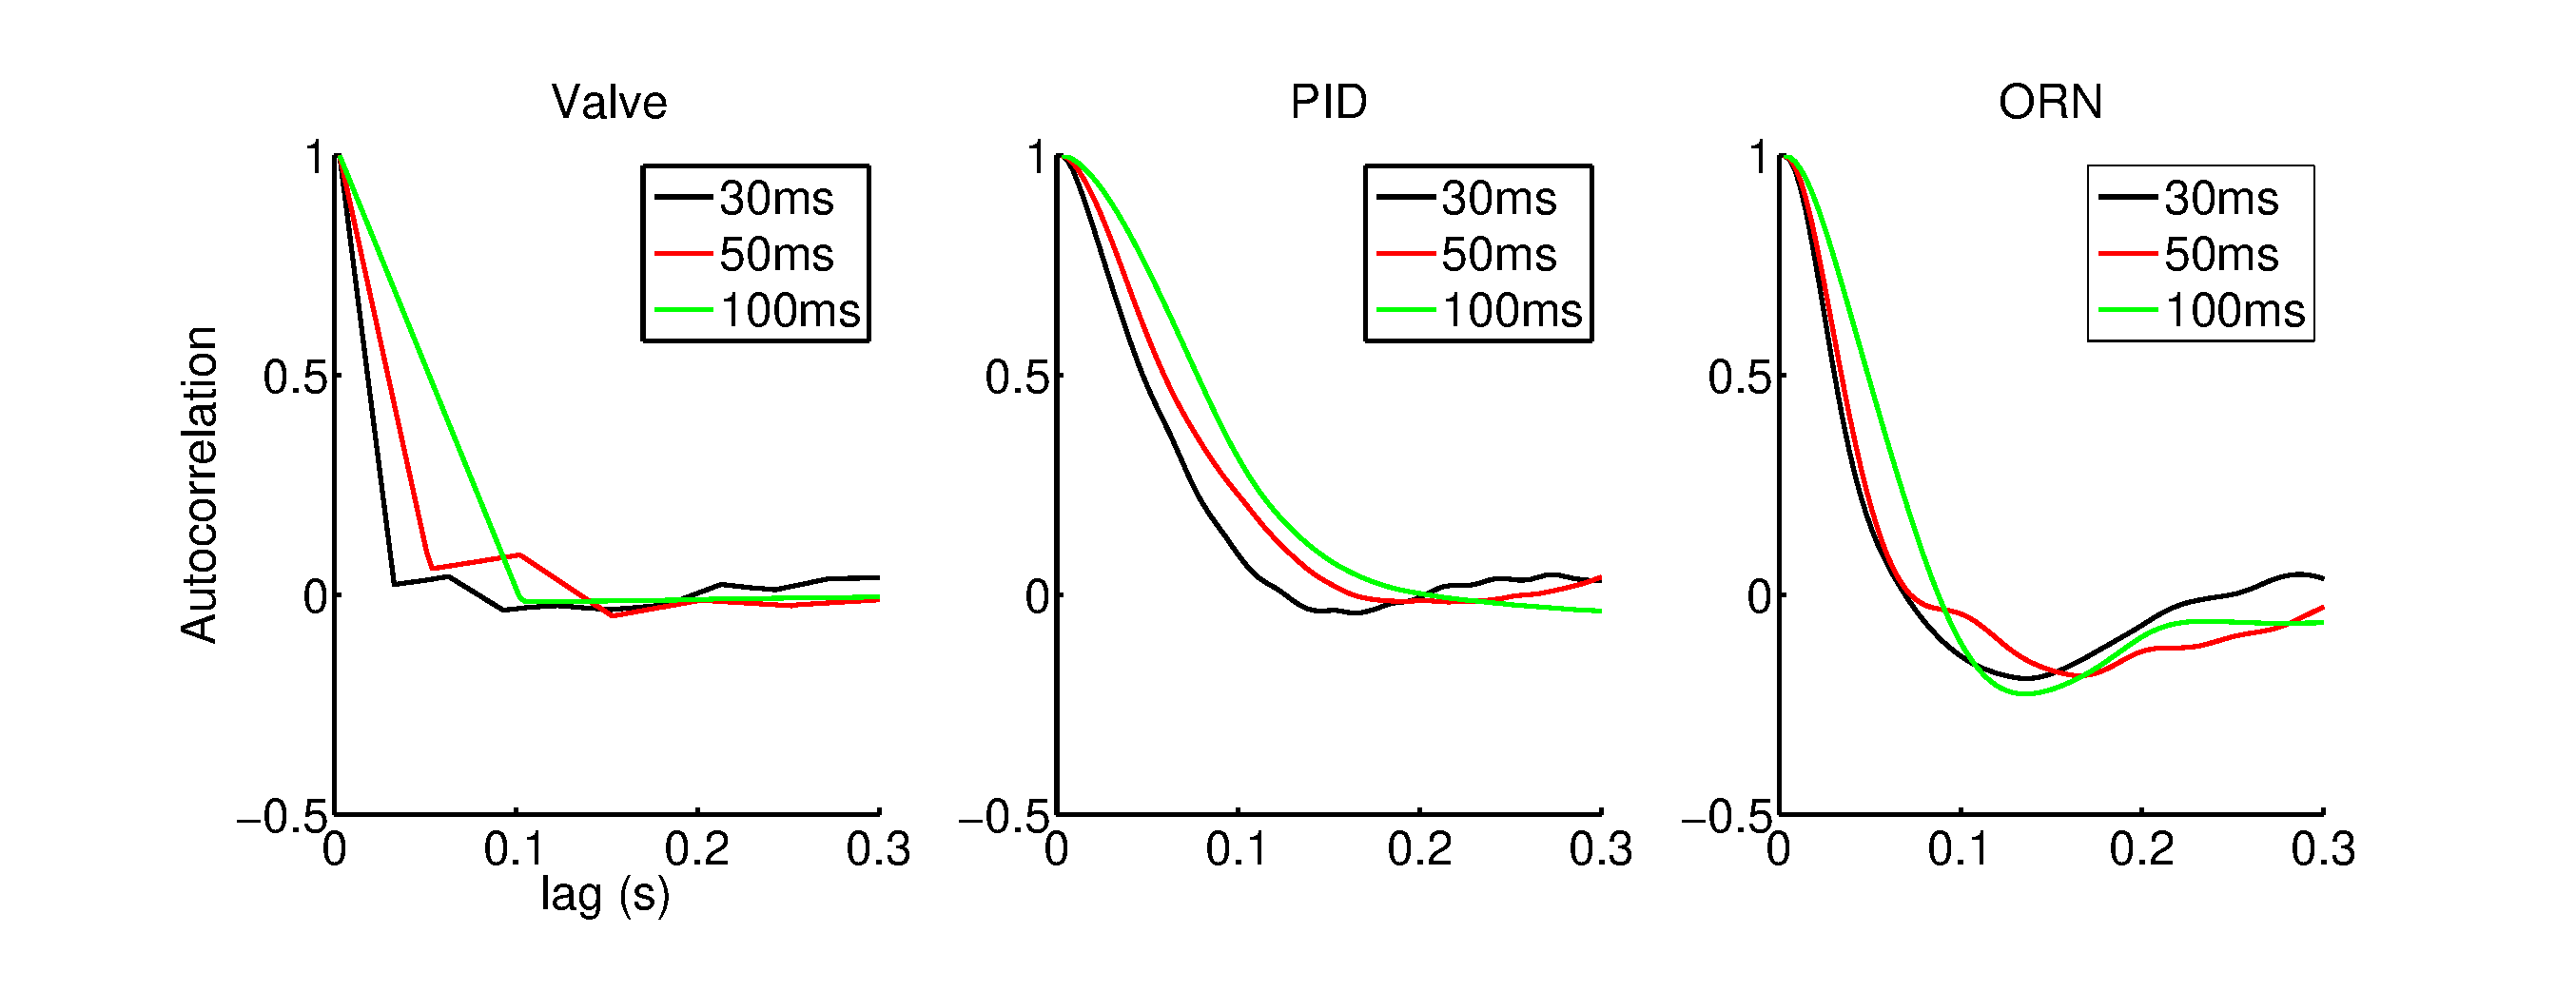
\includegraphics [width=\textwidth]{EffectOfCorrelationTime_01.pdf}
\begin{par}
Now we fit filters to these data sets. In the figure below, the filters on the left are calculated using a fixed regularisation (of 1), and the filters on the right, the regularisation is varied in each case to find the "best" filter, minimising errors, high frequency components, and having a gain as close to unity as possible. In either case, we see the filters are slightly different for the three data sets; the correlation time of the stimulus seems to affect the filter we extract.
\end{par} \vspace{1em}

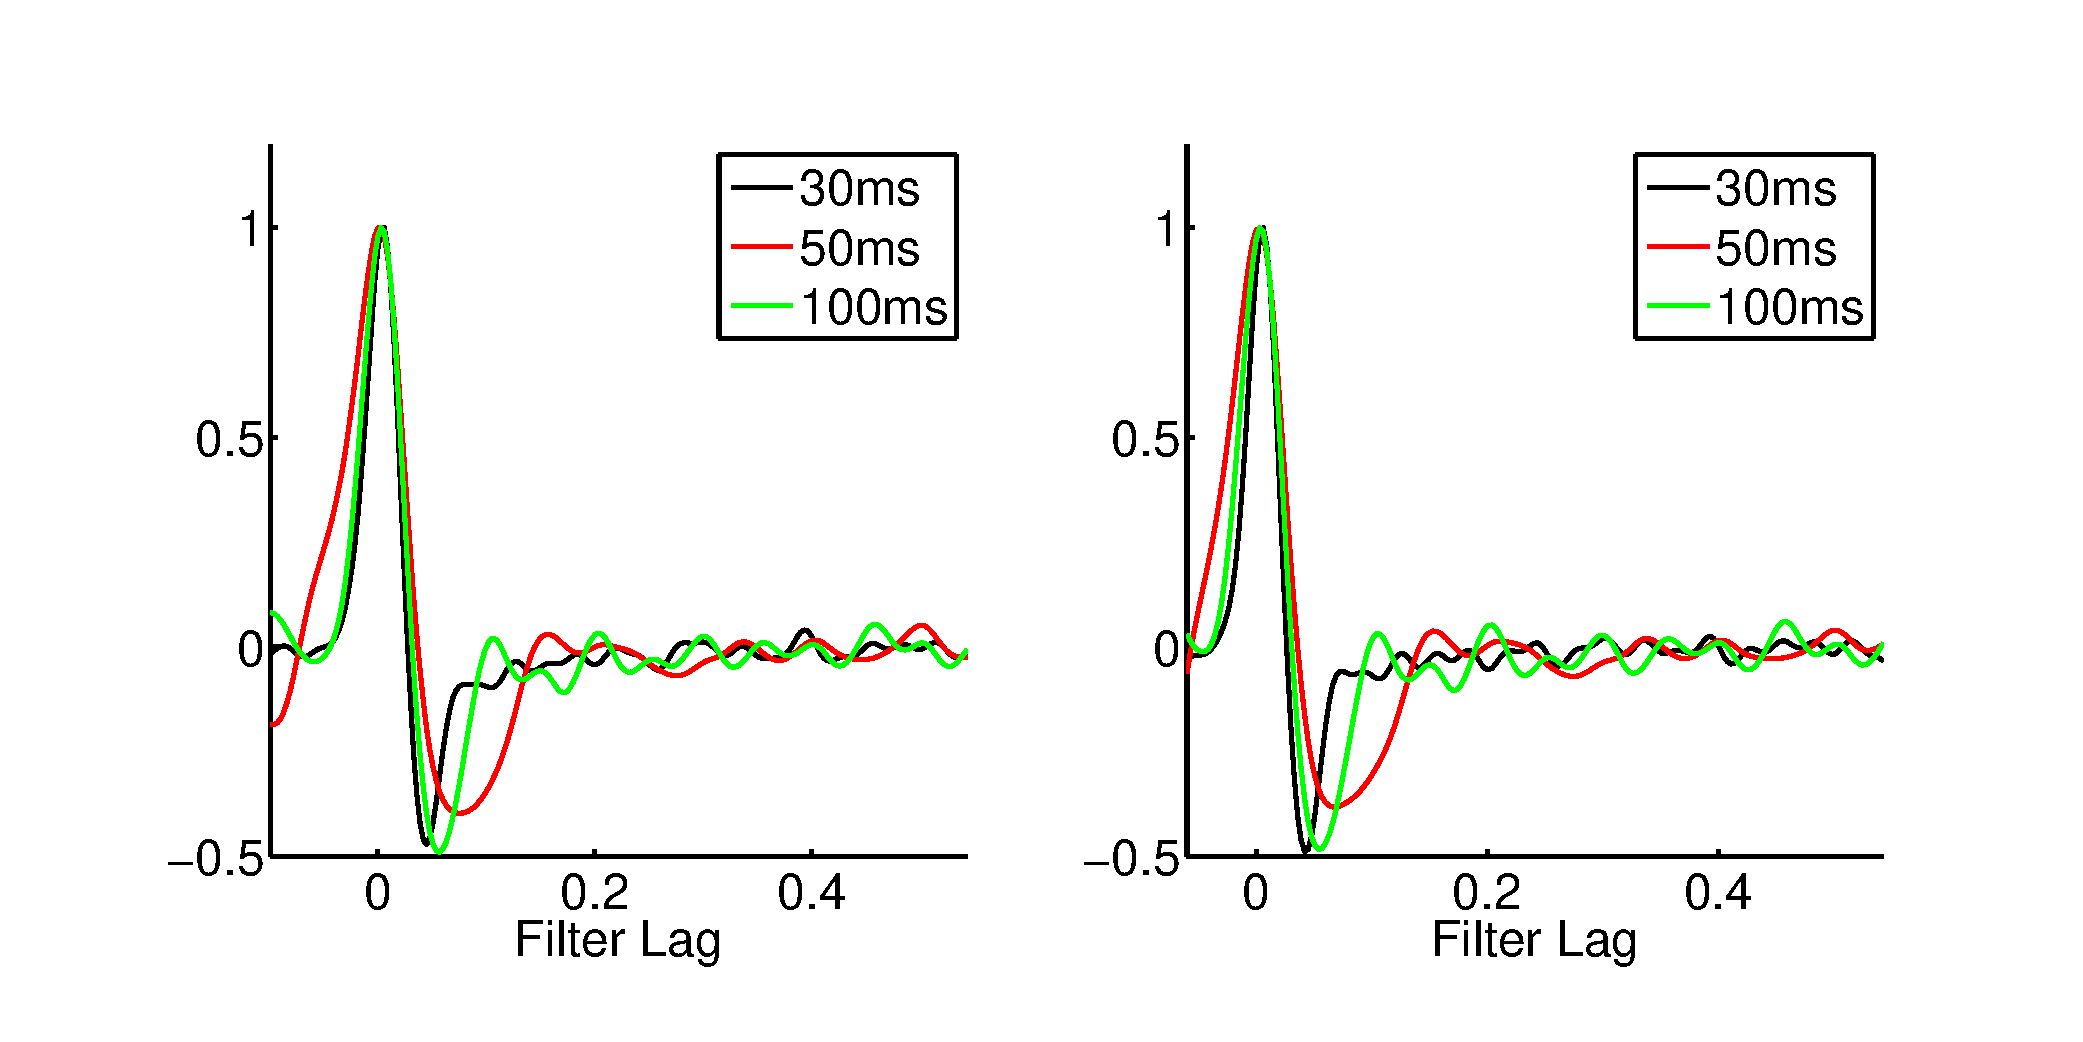
\includegraphics [width=\textwidth]{EffectOfCorrelationTime_02.pdf}
\begin{par}
How good are these filters at estimating the data? In the figure we below, we show the two extreme cases (the 30ms and 100ms correlated data) and the predictions from the filters calculated from their own data sets, along with predictions from filters calculated using the others' data.
\end{par} \vspace{1em}

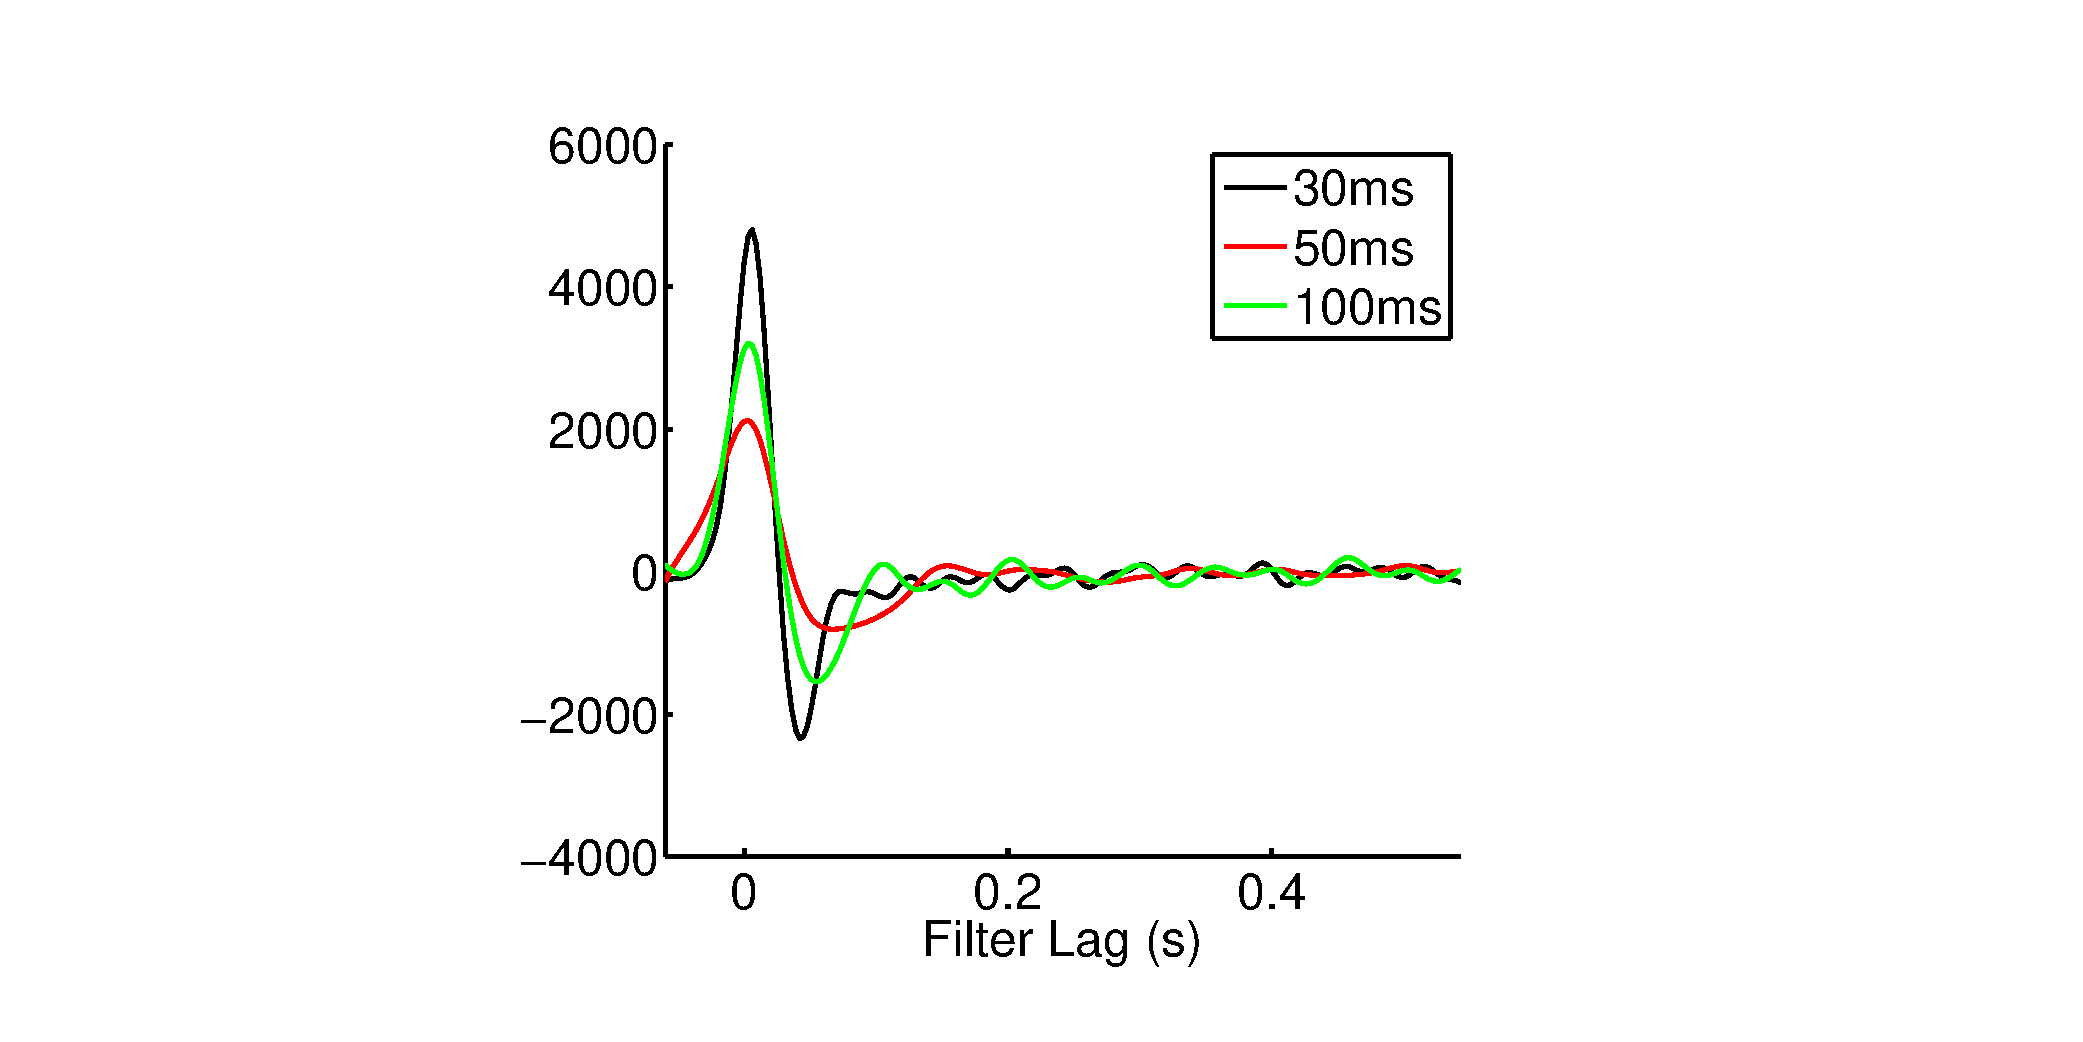
\includegraphics [width=\textwidth]{EffectOfCorrelationTime_03.pdf}
\begin{par}
How good are these cross-predictions? For the three data sets we have, we measure how well the filter from each data set predicts the data. In the matrix below, the element in ith row and jth column shows the r-square of linear prediction by the ith filter to jth data set, where the first data set has 30ms correlated stimulus, the second has 50ms correlated stimulus, and the 3rd has 100ms correlated stimulus.
\end{par} \vspace{1em}

        \color{lightgray} \begin{verbatim}    0.9344    0.9638    0.9424
    0.8271    0.9486    0.8788
    0.8991    0.9601    0.9397

\end{verbatim} \color{black}
    \begin{par}
In particular, predictions using the fastest filter outperform predictions even from filters from the same data set.
\end{par} \vspace{1em}



\end{document}
    
